\documentclass{article}
\usepackage{listings}
\usepackage{xcolor}
\usepackage{graphicx}

\definecolor{codegreen}{rgb}{0,0.6,0}
\definecolor{codegray}{rgb}{0.5,0.5,0.5}
\definecolor{codepurple}{rgb}{0.58,0,0.82}
\definecolor{backcolour}{rgb}{0.95,0.95,0.92}

\lstdefinestyle{mystyle}{
	backgroundcolor=\color{backcolour},
	commentstyle=\color{codegreen},
	keywordstyle=\color{magenta},
	numberstyle=\tiny\color{codegray},
	stringstyle=\color{codepurple},
	basicstyle=\footnotesize,
	breakatwhitespace=false,
	breaklines=true,
	captionpos=b,
	keepspaces=true,
	numbers=left,
	numbersep=5pt,
	showspaces=false,
	showstringspaces=false,
	showtabs=false,
	tabsize=2
}

\lstset{style=mystyle}

\title{I-ésimo Término de Tribonacci (Problema 7)}



\begin{document}
	
	\maketitle
	
	\section{Descripcion del Ejercicio}
	
	
	La sucesión recurrente de Tribonacci se define por la función $T(n)$, con $n \geq 0$ donde:
	\begin{itemize}
		\item $F(0) = 0$
		\item $F(1) = 0$
		\item $F(2) = 1$
		\item $F(n) = F(n-1) + F(n-2) + F(n-3)$
	\end{itemize}
	
	Dado un número $i$, hallar el $i$-ésimo término de la sucesión Tribonacci.
	
	\subsection*{Salida}
	
	Imprimir el $i$-ésimo término de Tribonacci, es decir, $T(i)$.
	
	Por ejemplo: Para $i=6$
	
	\textbf{Debería imprimir:}
	
	7
	
	\section*{Logisim}
	
	Se dispondrá en \textit{INPUT} los datos de entrada a partir de la dirección $0$. La entrada se estructura de la siguiente forma:
	
	\begin{itemize}
		\item $w_0$ : $i$
	\end{itemize}
	
	\section*{SASM}
	
	En la sección \texttt{.data} se deben definir los valores de entrada de la siguiente forma:
	
	\begin{verbatim}
		i dw 6
	\end{verbatim}
	
	\section{Pseudocódigo}
	
	\begin{lstlisting}[language=Python, caption=Función Tribonacci en Python]
		def Tribonacci(n):
		b = 0
		c = 0 
		a = 1
		while ( n > 2):
			a = a+b+c
			c,b = b,c
			b,a = a,b
			n = n-1
		if( a <= 1)
			a = 0
		return a
		
	\end{lstlisting}
	
	\section{Código en Ensamblador}
	
	\begin{lstlisting}[language={[x86masm]Assembler}, caption=Código Tribonacci en Ensamblador]
		%include "io.inc"
		
		section .data
		i dw 6
		
		section .text
		global main
		main:
		mov ebp, esp; for correct debugging 
		mov eax, 1 ; valor mas actual f(n-1)
		mov ebx, 0 ; valor anterior f(n-2)
		mov edx, 0 ; valor mas anterior f(n-3)
		
		xor ecx, ecx ; inicializa en 0 ecx
		
		movzx ecx, word [i] ; guarda el valor de i en ecx
		;mov ecx, i 
		
		; Aqui se definen los casos bases si ecx es 0 o 1 => 0, si ecx es 2=>1
		cmp ecx, 1 ; compara ecx con 1
		jle .base ; si es menor igual que 1
		
		cmp ecx, 2 ; compara ecx con 2
		je .end ;si es igual a 2
		
		; Si es mayor que 2, es decir no entra en los casos bases
		sub ecx, 2 ; resto 2 para quedarme con la cantidad de veces que debo ejecutar el codigo
		jmp .trib ; entra al bloque de codigo del tribonacci
		
		
		.base:
		mov eax, 0
		jmp .end
		
		.trib:
		add edx, eax ; sumar edx con eax y guardarlo en edx
		add edx, ebx ; sumar ebx con edx y guardarlo en edx
		
		; Esto permite dejar el valor de la ultima suma en orden de prioridad y eliminar el valor anterior
		xchg edx, ebx ; intercambiar los valores edx y ebx
		xchg ebx, eax ; intercambiar los valores ebx y eax
		
		; Decrementar el contador de las veces que debia ejecutar el codigo y comparar con 0
		; si es 0 ya terminamos y sale hasta .end si aun quedan veces por ejecutar salta nuevamente
		; al inicio del trib a ejecutar otra vez
		dec ecx
		cmp ecx, 0
		je .end
		
		jmp .trib
		
		.end:
		PRINT_DEC 1, eax
		
		xor eax, eax
		ret
	\end{lstlisting}
	 Para guardar el valor de i q tiene una extension de 16 bits en un ecx de 32 bits se utiliza la instrucción movzx que extiende ceros para llenar los bits de ecx.
	 
	\section{Diagrama de la Máquina de Estado}
	
	Para visualizar la máquina de estado, se incluye a continuación el diagrama correspondiente:
	
	\begin{figure}[h]
		\centering
		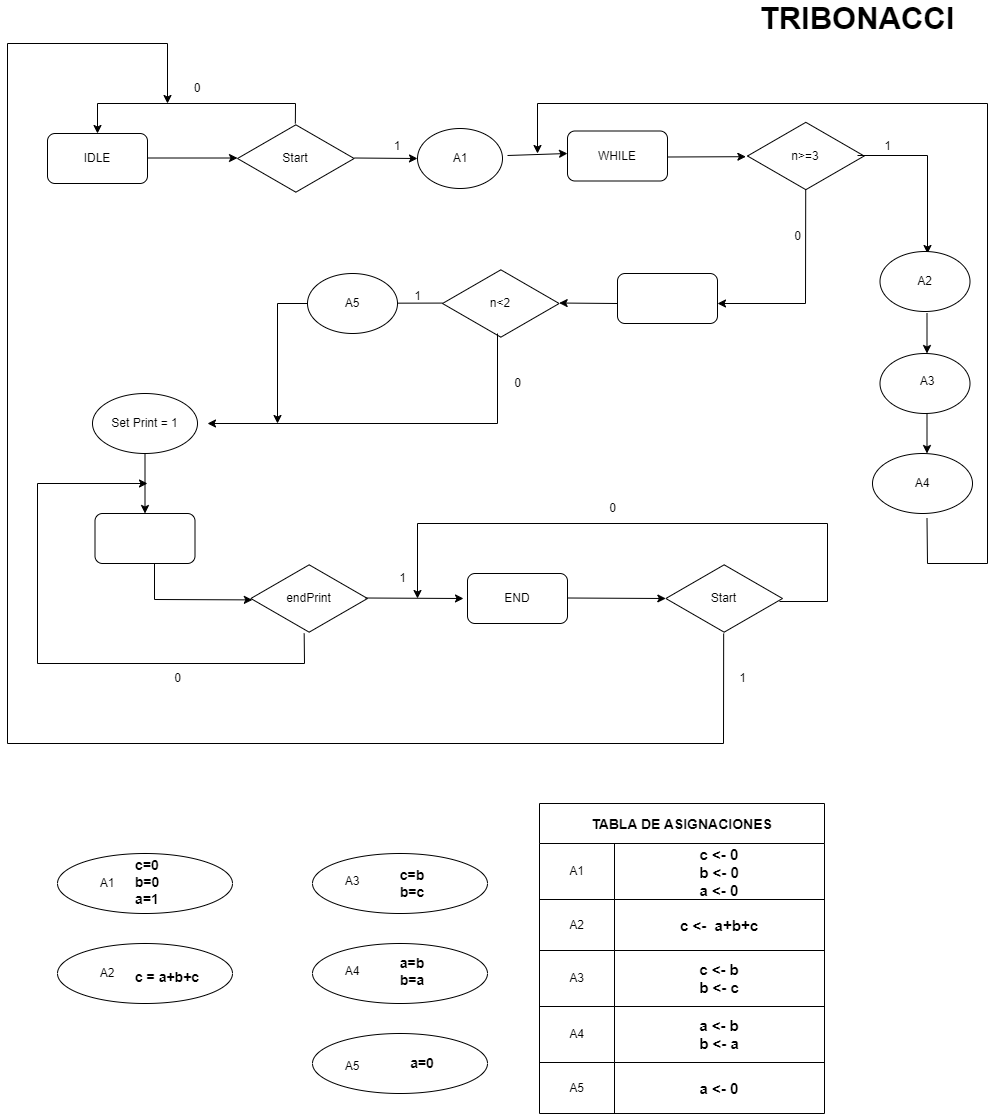
\includegraphics[width=0.9\textwidth]{Diagrama_Tribonacci.png}
		\caption{Diagrama de la máquina de estado.}
	\end{figure}
	
\end{document}
